%\documentclass[16p5,a4paper]{report}
\documentclass[14pt,a4paper]{report}
\usepackage[paperwidth=21cm, paperheight=29cm, left=3.5cm,right=2cm,top=3.5cm,bottom=3.0cm]{geometry}
\usepackage{xcolor}
\definecolor{ocre}{RGB}{243,102,25} 
\usepackage{filecontents}
\usepackage[utopia]{mathdesign} 
\usepackage{times}
\usepackage{mathptmx}
\usepackage{microtype} 
\usepackage{wallpaper} 
\usepackage{multirow} 
\DeclareGraphicsRule{*}{mps}{*}{}
\usepackage{ifthen}
\usepackage{calculator}
\usepackage{calc}
\usepackage{makeidx} 
\makeindex 


%----------------------------------------------------------------------------------------

\usepackage{titlesec} % cho phép điều chỉnh tiêu đề
\usepackage{graphicx}
\usepackage{tikz} 
\usepackage[utf8]{inputenc}
\usepackage[russian,vietnam]{babel}
\usepackage[T2A,T5]{fontenc}
\usepackage{array}
\usepackage{algorithm}
\usepackage{algorithmic}
% Dùng để nhập tiêng Nga

\usepackage[scaled=0.9]{PTSerif}
\usepackage[scaled=0.9]{PTSans}
\usepackage[scaled=0.87]{PTMono}
 
\usepackage{tgtermes}
\usepackage[scale=.90]{tgheros}
\usepackage{tgcursor}
 

\usepackage{substitutefont}
\substitutefont{T2A}{\rmdefault}{PTSerif-TLF}
\substitutefont{T2A}{\sfdefault}{PTSans-TLF}
\substitutefont{T2A}{\ttdefault}{PTMono-TLF}

% Hết dùng để nhập tiêng Nga

\usepackage{enumitem} 
\setlist{nolistsep} 

\usepackage{booktabs} % Để có đường thẳng ngang đẹp trong bảng

\usepackage{eso-pic} 

%----------------------------------------------------------------------------------------
% TABLE OF CONTENTS
%----------------------------------------------------------------------------------------

\usepackage{titletoc} 
\contentsmargin{0cm}
\titlecontents{chapter}[3.0cm] 
{\addvspace{15pt}\large\sffamily\bfseries} 
{\color{ocre!60}\contentslabel[\Large\thecontentslabel]{3.0cm}\color{ocre}} % Chapter number
{}  
{\color{ocre!60}\normalsize\sffamily\bfseries\;\titlerule*[.5pc]{.}\;\thecontentspage} 
\titlecontents{section}[3.0cm] 
{\addvspace{5pt}\sffamily\bfseries}
{\contentslabel[\thecontentslabel]{3.0cm}} 
{}
{\sffamily\hfill\color{black}\thecontentspage}
[]

\titlecontents{subsection}[3.0cm] 
{\addvspace{1pt}\sffamily\small}
{\contentslabel[\thecontentslabel]{3.0cm}} 
{}
{\sffamily\;\titlerule*[.5pc]{.}\;\thecontentspage}
[] 

%font
%----------------------------------------------------------------------------------------
% 	Bảng mục lục mini trên tiêu đề chương
%----------------------------------------------------------------------------------------


\titlecontents{lsection}[1em] 
{\footnotesize\sffamily} {}{}{}

\titlecontents{lsubsection}[.7em]
{\normalfont\footnotesize\sffamily} {}{}{}
 
%----------------------------------------------------------------------------------------
% 	PAGE HEADERS
%----------------------------------------------------------------------------------------

\usepackage{fancyhdr} 

\pagestyle{fancy}
\renewcommand{\chaptermark}[1]{\markboth{\sffamily\normalsize\bfseries #1}{}} 
\renewcommand{\sectionmark}[1]{\markright{\sffamily\normalsize\thesection\hspace{5pt}#1}{}} 
\fancyhf{} \fancyhead[LE,RO]{\sffamily\normalsize\thepage}
\fancyhead[LO]{\rightmark} 
\fancyhead[RE]{\leftmark}
\renewcommand{\headrulewidth}{0.5pt} 
\addtolength{\headheight}{2.5pt}
\renewcommand{\footrulewidth}{0pt}
\fancypagestyle{plain}{\fancyhead{}\renewcommand{\headrulewidth}{5pt}} 


\makeatletter
\renewcommand{\cleardoublepage}{
\clearpage\ifodd\c@page\else
\hbox{}
\vspace*{\fill}
\thispagestyle{empty}
\newpage
\fi}

%----------------------------------------------------------------------------------------
%	 THEOREM STYLES
%----------------------------------------------------------------------------------------
\let\circledS\undefined % here - PS
\usepackage{amsmath,amsfonts,amssymb,amsthm}
\newcommand{\intoo}[2]{\mathopen{]}#1\,;#2\mathclose{[}}
\newcommand{\ud}{\mathop{\mathrm{{}d}}\mathopen{}}
\newcommand{\intff}[2]{\mathopen{[}#1\,;#2\mathclose{]}}
\newtheorem{notation}{Notation}[chapter]


\newtheoremstyle{ocrenumbox}{0pt}{0pt}{\normalfont}{}
{\small\bf\sffamily\color{ocre}}
{\;}
{0.25em}
{\small\sffamily\color{ocre}\thmname{#1}\nobreakspace\thmnumber{\@ifnotempty{#1}{}\@upn{#2}}
\thmnote{\nobreakspace\the\thm@notefont\sffamily\bfseries\color{black}---\nobreakspace#3.}} 
\renewcommand{\qedsymbol}{$\blacksquare$}

\newtheoremstyle{blacknumex}
{5pt}
{5pt}
{\normalfont}
{} 
{\small\bf\sffamily}
{\;}
{0.25em}
{\small\sffamily{\tiny\ensuremath{\blacksquare}}\nobreakspace\thmname{#1}\nobreakspace\thmnumber{\@ifnotempty{#1}{}\@upn{#2}}
\thmnote{\nobreakspace\the\thm@notefont\sffamily\bfseries---\nobreakspace#3.}}

\newtheoremstyle{blacknumbox} {0pt}{0pt}{\normalfont}{}{\small\bf\sffamily}{\;}{0.25em}
{\small\sffamily\thmname{#1}\nobreakspace\thmnumber{\@ifnotempty{#1}{}\@upn{#2}}\thmnote{\nobreakspace\the\thm@notefont\sffamily\bfseries---\nobreakspace#3.}}


\newtheoremstyle{ocrenum}{5pt}{5pt}{\normalfont}{}{\small\bf\sffamily\color{ocre}}{\;}{0.25em}{\small\sffamily\color{ocre}\thmname{#1}\nobreakspace\thmnumber{\@ifnotempty{#1}{}\@upn{#2}}
\thmnote{\nobreakspace\the\thm@notefont\sffamily\bfseries\color{black}---\nobreakspace#3.}}
\renewcommand{\qedsymbol}{$\blacksquare$}
\makeatother


\newcounter{dummy} 
\numberwithin{dummy}{section}
\theoremstyle{ocrenumbox}
\newtheorem{theoremeT}[dummy]{Định lý }
\newtheorem{problem}{Bài toán}[chapter]
\newtheorem{exerciseT}{Bài tập}[chapter]
\theoremstyle{blacknumex}
\newtheorem{exampleT}{Ví dụ}[chapter]
\theoremstyle{blacknumbox}
\newtheorem{vocabulary}{Vocabulary}[chapter]
\newtheorem{definitionT}{Định nghĩa }[section]
\newtheorem{corollaryT}[dummy]{Hệ quả}
\theoremstyle{ocrenum}
\newtheorem{proposition}[dummy]{Proposition}

%----------------------------------------------------------------------------------------
%	 Định nghĩa các cái hộp viền màu và tô màu
%----------------------------------------------------------------------------------------

\RequirePackage[framemethod=default]{mdframed}

% Hộp Định lý
\newmdenv[skipabove=7pt,
skipbelow=7pt,
backgroundcolor=black!5,
linecolor=ocre,
innerleftmargin=5pt,
innerrightmargin=5pt,
innertopmargin=5pt,
leftmargin=0cm,
rightmargin=0cm,
innerbottommargin=5pt]{tBox}

%  Hộp bài tập
\newmdenv[skipabove=7pt,
skipbelow=7pt,
rightline=false,
leftline=true,
topline=false,
bottomline=false,
backgroundcolor=ocre!10,
linecolor=ocre,
innerleftmargin=5pt,
innerrightmargin=5pt,
innertopmargin=5pt,
innerbottommargin=5pt,
leftmargin=0cm,
rightmargin=0cm,
linewidth=4pt]{eBox}	

% Định nghĩa cái hộp
\newmdenv[skipabove=7pt,
skipbelow=7pt,
rightline=false,
leftline=true,
topline=false,
bottomline=false,
linecolor=ocre,
innerleftmargin=5pt,
innerrightmargin=5pt,
innertopmargin=0pt,
leftmargin=0cm,
rightmargin=0cm,
linewidth=4pt,
innerbottommargin=0pt]{dBox}	

% Hộp hệ quả
\newmdenv[skipabove=7pt,
skipbelow=7pt,
rightline=false,
leftline=true,
topline=false,
bottomline=false,
linecolor=gray,
backgroundcolor=black!5,
innerleftmargin=5pt,
innerrightmargin=5pt,
innertopmargin=5pt,
leftmargin=0cm,
rightmargin=0cm,
linewidth=4pt,
innerbottommargin=5pt]{cBox}				  
		  

% Tạo môi trường cho mỗi loại Định lý
\newenvironment{theorem}{\begin{tBox}\begin{theoremeT}}{\end{theoremeT}\end{tBox}}
\newenvironment{exercise}{\begin{eBox}\begin{exerciseT}}{\hfill{\color{ocre}\tiny\ensuremath{\blacksquare}}\end{exerciseT}\end{eBox}}				  
\newenvironment{definition}{\begin{dBox}\begin{definitionT}}{\end{definitionT}\end{dBox}}	
\newenvironment{example}{\begin{exampleT}}{\hfill{\tiny\ensuremath{\blacksquare}}\end{exampleT}}		
\newenvironment{corollary}{\begin{cBox}\begin{corollaryT}}{\end{corollaryT}\end{cBox}}	

%----------------------------------------------------------------------------------------
% 	REMARK ENVIRONMENT
%----------------------------------------------------------------------------------------

\newenvironment{remark}{\par\vskip10pt\small \begin{list}{}{\leftmargin=35pt
\rightmargin=25pt}\item\ignorespaces 
\makebox[-2.5pt]{\begin{tikzpicture}[overlay]
\node[draw=ocre!60,line width=1pt,circle,fill=ocre!25,font=\sffamily\bfseries,inner sep=2pt,outer sep=0pt] at (-15pt,0pt){\textcolor{ocre}{Nh\d{\^a}n x\'et}};\end{tikzpicture}} % Orange R in a circle
\advance\baselineskip -1pt}{\end{list}\vskip5pt}

%----------------------------------------------------------------------------------------
%	 SECTION NUMBERING IN THE MARGIN
%----------------------------------------------------------------------------------------

\makeatletter
\renewcommand{\@seccntformat}[1]{\llap{\textcolor{ocre}{\csname the#1\endcsname}\hspace{1em}}}      
\renewcommand{\section}{\@startsection{section}{1}{\z@}
{-3.5ex \@plus -1ex \@minus -.2ex}
{2.3ex \@plus.2ex }
{\normalfont\large\sffamily\bfseries}}
\renewcommand{\subsection}{\@startsection {subsection}{2}{\z@}
{-3.25ex \@plus -1ex \@minus -.2ex}
{1.5ex \@plus.2ex }
{\normalfont\sffamily\bfseries}}
\renewcommand{\subsubsection}{\@startsection {subsubsection}{3}{\z@}
{-3.25ex \@plus -1ex \@minus -.2ex}
{1.5ex \@plus.2ex }
{\normalfont\small\sffamily\bfseries}}                        
\renewcommand\paragraph{\@startsection{paragraph}{4}{\z@}
{-3.25ex \@plus-.2ex \@minus .2ex}
{-1em}
{\normalfont\small\sffamily\bfseries}}



                                     
                                                    
%----------------------------------------------------------------------------------------
% Tiêu đề chương
%----------------------------------------------------------------------------------------

\newcommand{\thechapterimage}{}
\newcommand{\chapterimage}[1]{\renewcommand{\thechapterimage}{#1}}
\def\thechapter{\arabic{chapter}}
\def\@makechapterhead#1{
\thispagestyle{empty}
{\centering \normalfont\sffamily
\ifnum \c@secnumdepth >\m@ne
\if@mainmatter
\startcontents
\begin{tikzpicture}[remember picture,overlay]
\node at (current page.north west)
{\begin{tikzpicture}[remember picture,overlay]

\node[anchor=north west,inner sep=0pt] at (0,0) {\includegraphics[width=\paperwidth]{\thechapterimage}};

%Commenting the 3 lines below removes the small contents box in the chapter heading
\draw[fill=white,opacity=.6] (1.55cm,0) rectangle (7cm,-7cm);
\node[anchor=north west] at (2cm,.25cm) {\parbox[t][8cm][t]{6.5cm}{\huge\bfseries\flushleft \vspace*{2cm}\printcontents{l}{1}{\setcounter{tocdepth}{1}}}};

\draw[anchor=west] (4cm,-5cm) node [rounded corners=25pt,fill=white,fill opacity=.6,text opacity=1,draw=ocre,draw opacity=1,line width=2pt,inner sep=15pt]{\huge\sffamily\bfseries\textcolor{black}{\thechapter\ --\ #1\vphantom{plPQq}\makebox[15cm]{}}};  %22cm -9cm
\end{tikzpicture}};
\end{tikzpicture}}\par\vspace*{230\p@}
\fi
\fi
}
\def\@makeschapterhead#1{
\thispagestyle{empty}
{\centering \normalfont\sffamily
\ifnum \c@secnumdepth >\m@ne
\if@mainmatter
\startcontents
\begin{tikzpicture}[remember picture,overlay]
\node at (current page.north west)
{\begin{tikzpicture}[remember picture,overlay]
\node[anchor=north west] at (-4pt,4pt) {\includegraphics[width=\paperwidth]{\thechapterimage}};
\draw[anchor=west] (5cm,-5cm) node [rounded corners=25pt,fill=white,opacity=.7,inner sep=15.5pt]{\huge\sffamily\bfseries\textcolor{black}{\vphantom{plPQq}\makebox[15cm]{}}};
\draw[anchor=west] (5cm,-5cm) node [rounded corners=25pt,draw=ocre,line width=2pt,inner sep=15pt]{\huge\sffamily\bfseries\textcolor{black}{#1\vphantom{plPQq}\makebox[15cm]{}}};
\end{tikzpicture}};
\end{tikzpicture}}\par\vspace*{250\p@}
\fi
\fi
}
\makeatother


\begin{document}
\fontsize{13.5}{18}\selectfont

\parindent=0pt
\newcommand*\varhrulefill[1][0.4pt]{\leavevmode\leaders\hrule height#1\hfill\kern0pt}

\title{Toán rời rạc}

\chapterimage{chapter_head_1.pdf} 
\pagestyle{empty}
\tableofcontents
\listoffigures 
\listoftables
\cleardoublepage
\pagestyle{fancy}
\renewcommand\indexname{INDEX}
%----------------------------------------------------------------------------------------
% 	CHAPTER 1
%----------------------------------------------------------------------------------------
\everymath{\displaystyle}
\newcommand{\vt}[1]{\overrightarrow{#1}}
\newcommand{\vecto}{vectơ\ }
\newcommand{\Vecto}{Vectơ\ }
\newcommand{\tch}[2]{\left[\vt{#1},\vt{#2}\right]}
\newcommand{\Tch}[2]{\left[#1,#2\right]}
\newcommand{\dinhthuc}[4]{\left|\begin{array}{cc}
#1 & #2 \\ 
#3 & #4
\end{array} \right|}

\newcommand{\dthai}[4]{\left|\begin{array}{cc}
#1 & #2 \\ 
#3 & #4
\end{array} \right|}

\newcommand{\dtba}[9]{\left|\begin{array}{ccc}
#1 & #2 &#3 \\ 
#4 & #5 &#6 \\ 
#7 & #8 &#9  
\end{array} \right|}


\newcommand{\tinhdtba}[9]{\DETERMINANT(#1,#2,#3;#4,#5,#6;#7,#8,#9){\sol}
\left|\begin{array}{ccc}
#1 & #2 &#3 \\ 
#4 & #5 &#6 \\ 
#7 & #8 &#9  
\end{array} \right|=\sol
}

\newcommand{\tdtba}[9]{\DETERMINANT(#1,#2,#3;#4,#5,#6;#7,#8,#9){\sol}
\sol
}

\newcommand{\tdthai}[4]{\DETERMINANT(#1,#2;#3,#4){\sol}\sol
}

\newcommand{\khung}[2]{\begin{tabular}{|c|}
\hline 
\parbox{#1}{{\color{white}{a}}\\ #2} \\ 
\hline 
\end{tabular}\bigskip \\  }


\newcommand*\circled[1]{\tikz[baseline=(char.base)]{
  \node[shape=circle,draw,inner sep=2pt] (char) {#1};}}

\chapterimage{chapter_head_2a.pdf} % Chapter heading image

\chapter{Giới thiệu về giải thuật GRASP\index{GRASP}}

\section{Giới thiệu\index{GRASP}}
GRAPS\index{GRASP} (Greedy Randomized Adaptive Search Procedure) là một metaheuristic đa khởi đầu để giải quyết các vấn đề tối ưu tổ hợp khó khăn. Mỗi lần lặp của GRASP bao gồm 2 giai đoạn: 1 giai đoạn xây dựng cấu trúc tham ăn thích nghi ngẫu nhiên và một giai đoạn tìm kiếm địa phương (local search\index{local search}). Bắt đầu từ các giải pháp khả thi được xây dựng từ giai đoạn tìm cấu trúc tham lam thích nghi ngẫu nhiên, giai đoạn tìm kiếm địa phương sẽ tìm kiếm các giải pháp hàng xóm của giải pháp được chọn cho đến khi tìm được một giải pháp tối ưu địa phương. Giải pháp tốt nhất được tìm thấy qua tất cả các lần lặp được là kết quả của quá trình.\\

GRAPS được giới thiệu lần đầu tiên vào năm 1989 bởi Thomas A. Feo và Mauricio G. C. Resende. Trong lần giới thiệu đầu tiên này GRASP đã được ứng dụng vào vấn đề tập phủ.\\


\section{Bài toán và giải thuật}
Xét bài toán tối ưu tổ hợp định nghĩa bởi một tập hữu hạn $E$ = {1,...,n}, một tập tất cả các giải pháp có thể $F\subseteq 2^E$ và một hàm mục tiêu $f$: $2^E \rightarrow$ $R$. Trong phiên bản cực tiểu, chúng ta tìm một giải pháp $S^* \in F$ sao cho $f(S^*) \leq f(S), \forall S \in F$. Tập $E$, hàm giá $f$, tập các giải pháp khả thi $F$ được định nghĩa cụ thể cho từng bài toán. Ví dụ, trong trường hợp của bài toán người đi du lịch, tập $E$ là tập tất cả các cạnh kết nối tất cả các thành phố cần được tới thăm. Hàm giá $f(S)$ là tổng giá trị của tất cả các cạnh $e \in S$, và $F$ được hình thành bởi tất cả các tập cạnh xác định bởi chu trình Haminton.\\
GRAPS\index{GRASP} (Greedy Randomized Adaptive Search Procedure) là một metaheuristic đa khởi đầu để giải quyết các vấn đề tối ưu tổ hợp khó khăn. Mỗi lần lặp của GRASP bao gồm 2 giai đoạn: 1 giai đoạn xây dựng cấu trúc tham ăn thích nghi ngẫu nhiên và một giai đoạn tìm kiếm địa phương (local search\index{local search}). Bắt đầu từ các giải pháp khả thi được xây dựng từ giai đoạn tìm cấu trúc tham lam thích nghi ngẫu nhiên, giai đoạn tìm kiếm địa phương sẽ tìm kiếm các giải pháp hàng xóm của giải pháp được chọn cho đến khi tìm được một giải pháp tối ưu địa phương. Giải pháp tốt nhất được tìm thấy qua tất cả các lần lặp được là kết quả của quá trình. Giả mã trong hình 1.1 mô tả khối main của quá trình GRASP cho giá trị cực tiểu với Max\_Iterations bước lặp được thực hiện và Seed\index{Seed} được sử dụng như giá trị ban đầu cho hàm sinh số giả ngẫu nhiên.\\ \\

{\bf procedure} \texttt{GRASP(Max\_Iterations, Seed)}
\begin{algorithmic} [1] 
	\STATE \texttt{Read\_Input()};
	\FOR {$k=1$ \TO \texttt{Max\_Iterations}}
	\STATE \texttt{Solution} $\leftarrow$ \texttt{Greedy\_Randomized\_Construction(Seed)};
	\STATE \texttt{Solution} $\leftarrow$ \texttt{Local\_Search(Solution)};
	\STATE \texttt{Update\_Solution(Solution, Best\_Solution)};
	\ENDFOR
	\STATE {\bf return} \texttt{Best\_Solution};
\end{algorithmic}
{\bf end} \texttt{GRASP.}\\

Bên dưới là giả mã của quá trình xây dựng  cấu trúc tham lam thích nghi ngẫu nhiên. Với mỗi lần lặp lại giai đoạn này, tập các ứng cử viên được hình thành từ tất cả các phần tử có thể kết hợp với một giải pháp cụ thể mà không làm mất tính khả thi. Việc lựa chọn các phần tử tiếp theo để tổng hợp được xác định bởi việc đánh giá tất cả các ứng cử viên theo một hàm đánh giá tham lam. Hàm tham lam này thường đại diện cho chi phí do sự kết hợp của các ứng cử viên này vào các giải pháp được xây dựng. Việc đánh giá các phần tử này bằng hàm đánh giá dẫn đến việc tạo ra một danh sách ứng cử viên bị hạn chế (RLC\index{RCL} viết tắt của Restricted Candidate List) bởi các phần tử tốt nhất. Các phần tử kết hợp với giải pháp cụ thể hiện tại cho giá trị hàm giá tăng lên nhỏ nhất (đó là tính tham lam của thuật toán). Những phần tử này được lựa chọn ngẫu nhiên từ danh sách ứng cử viên hạn chế (đây là tính xác xuất hay ngẫu nhiên của thuật toán). Khi có một ứng cử viên được lựa chọn, danh sách ứng cử viên sẽ được cập nhật, giá trị gia tăng của hàm giá cũng được đánh giá lại (đây là tính thích nghi của thuật toán). Chiến lược này cũng tương tự như chiến lược bán tham lam của Hart và Shogan (1987), cũng là một giải pháp đa bắt đầu dựa trên cấu trúc tham lam ngẫu nhiên, nhưng không có tìm kiếm địa phương.\\

{\bf procedure} \texttt{Greedy\_Randomized\_Contruction(Seed)}
\begin{algorithmic} [1] 
	\STATE \texttt{Solution} $\leftarrow \emptyset$;
	\STATE Evaluate the incremental cost of candidate elements;
	\WHILE {\texttt{Solution} is not a complete solution}
	\STATE Build the restricted candidate list (RCL);
	\STATE Select an elment $s$ from the RCL at random;
	\STATE \texttt{Solution} $\leftarrow$ \texttt{Solution} $\cup \{s\}$;
	\STATE Reevaluate the incremental costs;
	\ENDWHILE
	\STATE {\bf return} \texttt{Solution};
\end{algorithmic}
{\bf end} \texttt{Greedy\_Randomized\_Contruction.}\\

Các giải pháp được sinh ra từ cấu trúc tham lam ngẫu nhiên không nhất thiết phải tối ưu, thậm chí là tối ưu đơn giản. Giai đoạn tìm kiếm địa phương thường sẽ cải thiện lại giải pháp đó. Một giải thuật tìm kiếm địa phương làm việc trong một bước lặp bằng cách liên tục thay thế giải pháp hiện tại bằng giải pháp lân cận tốt hơn của giải pháp hiện tại. Giả mã của thuật toán tìm kiếm địa phương bắt đầu từ giải pháp Solution của giai đoạn đầu tiên và sử dụng một N - hàng xóm được giữ như giả mã ở trên.\\

{\bf procedure} \texttt{Local\_Search(Solution)}
\begin{algorithmic} [1] 
	\WHILE {\texttt{Solution} is not locally optimal}
	\STATE Build the restricted candidate list (RCL);
	\STATE Find $s' \in N(\texttt{Solution})$ with $f(s') < f (\texttt{Solution})$;
	\STATE \texttt{Solution} $\leftarrow$ $s'$;
	\ENDWHILE
	\STATE {\bf return} \texttt{Solution};
\end{algorithmic}
{\bf end} \texttt{Local\_Search.}\\

Hiệu quả của một thủ tục tìm kiếm địa phương phụ thuộc vào một số khía cạnh như: cấu trúc của hàng xóm, kĩ thuật tìm kiếm hàng xóm, đánh giá nhanh của hàm giá của hàng xóm, và giải pháp bắt đầu của nó. Giai đoạn xây dựng giải pháp đóng vai trò quan trọng đối với các khía cạnh cuối cùng, xây dựng giải pháp bắt đầu có chất lượng cao cho tìm kiếm địa phương. Phương pháp hàng xóm đơn giản (simple neighborhoods) thường được sử dụng. Việc tìm kiếm hàng xóm có thể được thực hiện bằng cách sử dụng một cải tiến tốt nhất (best-improving \index{best-improving}) hoặc chiến lược cải tiến đầu tiên (first-improving\index{first-improving}). Trong trường hợp của chiến lược cải tiến tốt nhất, tất cả các hàng xóm được điều tra và hàng xóm tốt nhất được sử dụng. Trong trường hợp của chiến lược cải tiến đầu tiên, giải pháp hiện tại được chuyển tới giải pháp hàng xóm đầu tiên có giá trị hàm giá nhỏ hơn giá trị hiện tại. Trong thực hành, khi quan sát nhiều ứng dụng của cả hai chiến lược đều đưa tới cùng kết quả cuối cùng, nhưng chiến lược cải tiến đầu tiên thường cho thời gian tính toán nhỏ hơn.

\chapterimage{chapter_head_2a.pdf} % Chapter heading image

\chapter{Cấu trúc của danh sách ứng viên hạn chế}
\section{Cấu trúc của danh sách ứng viên hạn chế}
Một tính chất đặc biệt của GRASP là nó dễ dàng được thực hiện và cài đặt. Vài thông số cần phải được thiết lập và điều chỉnh. Vì vậy, phát triển thể
tập trung thực hiện các cấu trúc dữ liệu hiệu quả để đảm bảo lặp lại nhanh chóng. GRASP có hai thông số chính: một liên quan đến các tiêu chí dừng và một liên quan tới chất lượng của các yếu tố trong danh sách ứng cử viên bị hạn chế. Tiêu chí để dừng giải thuật được sử dụng trong giả mã thủ tục GRASP ở chương 1 được xác định là số Max\_Iterations các bước lặp. Mặc dù xác suất tìm được một giải pháp mới cải tiến tốt nhất với một số bước lặp, chất lượng của giải pháp tốt nhất được tìm thấy có thể chỉ cải thiện với các lần lặp sau. Từ khi thời gian tính toán qua từng bước lặp không thay đổi nhiều, tổng thời gian tính toán có thể dự doán được là tăng tuyến tính tới số lần lặp. Do đó, với một số lượng lớn các bước lặp, thời gian tính toán sẽ lớn hơn và kết quả tìm kiếm cũng tốt hơn.\\
Đối với việc xây dựng danh sách ứng viên hạn chế RCL được sử dụng trong giai đoạn đầu tiên, không làm mất tính tổng quát, một vấn đề cực tiểu như là một công thức trong mục 1.1. Ký hiệu $c(e)$ là giá trị gia tăng liên quan tới sự kết hợp của phần tử $e \in E$ tới cấu trúc của giải pháp. Tại mỗi bước lặp của GRASP, đặt
$c^min$ và $c^max$ là giá trị gia tăng nhỏ nhất và lớn nhất.\\

Danh sách ứng viên hạn chế RCL được tạo thành từ các phần tử $e \in E$ với giá trị gia tăng tốt nhất (i.e., nhỏ nhất) $c(e)$. Danh sách này có thể bị giới hạn bởi số lượng các phần tử (cardinality-based) hoặc bởi chất lượng của chúng (value-based). Trong trường hợp đầu tiên, danh sách RCL được tạo thành từ $p$ phần tử với giá trị gia tăng giá tốt nhất, $p$ ở đây là một tham số. Các danh sách RCL được liên kết tới một tham số ngưỡng $\alpha \in [0, 1]$. Danh sách ứng viên hạn chế được hình thành từ tất cả các phần tử $e in E$ có thể thêm vào cấu trúc của giải pháp cụ thể thêm vào danh sách cụ thể mà không làm mất tính khả thi của giải pháp đó và có chất lượng vượt trội giá trị ngưỡng, i.e., $c(e) \in [c^min, c^min + \alpha (c^max - c^min)]$. Trường hợp $\alpha$ = 0 tương ứng với giải thuật thuần tham lam. Giả mã phía dưới là một sàng lọc của giả mã cấu trúc tham lam thích nghi ngẫu nhiên trong thủ tục Greedy\_Randomized\_Contruction ở chương 1 và chỉ ra rằng tham số $\alpha$ điều khiển độ tham lam và tính ngẫu nhiên của thuật toán.\\

{\bf procedure} \texttt{Greedy\_Randomized\_Contruction($\alpha$, Seed)}
\begin{algorithmic} [1] 
	\STATE \texttt{Solution} $\leftarrow \emptyset$;
	\STATE Initialize the candidate set: $C \leftarrow E$;
	\STATE Evaluate the incremental cost $c(e)$ for all $e \in C$;
	\WHILE {$C \ne \emptyset$}
	\STATE $c\textsuperscript{min} \leftarrow $ min \{$c(e)\,|\, e \in C$\}
	\STATE $c\textsuperscript{max} \leftarrow $ max \{$c(e)\,|\, e \in C$\}
	\STATE {\bf RCL} $\leftarrow$ \{$e \in C\,|\, c(e) \lefteqn c\textsuperscript(min) + \alpha (c\textsuperscript{max} - c\textsuperscript{min})$\};
	\STATE Select an element $s$ from the RCL at random;
	\STATE \texttt{Solution} $\leftarrow$ \texttt{Solution} $\cup \{s\}$;
	\STATE Update the candidate set $C$;
	\STATE Reevaluate the incremental costs $c(e)$ for all $e \in C$;
	\ENDWHILE
	\STATE {\bf return} \texttt{Solution};
\end{algorithmic}
{\bf end} \texttt{Greedy\_Randomized\_Contruction.}\\

GRASP có thể được xem như một kỹ thuật lấy mẫu lặp đi lặp lại. Mỗi bước lặp tạo ra một mẫu giải pháp từ một phân phối không biết, trung bình và phương sai là chức năng và hạn chế tự nhiên của danh sách RCL. Ví dụ, nếu RCL được hạn chế bởi một phần tử duy nhất, thì các giải pháp tương tự cũng sẽ được tạo ra ở tất cả các bước lặp. Phương sai của phân phối sẽ tới 0 và trung bình sẽ tới giá trị của giải pháp tham lam. Nếu danh sách RCL có nhiều phần tử hơn, nhiều giải pháp khác nhau sẽ được tạo ra, phương sai sẽ lớn hơn. Từ khi tham lam đóng vai trò nhỏ trong trường hợp này, giá trị của giải pháp trung bình trở nên tồi hơn. Tuy nhiên, giá trị của giải pháp tốt nhất được tìm thấy nhanh hơn giá trị trung bình và thường là tối ưu. Biểu đồ trong hình 2.1 minh họa trường hợp này trong bài toán MAXSAT với 100 biến và 850 ràng buộc, kết quả thu được với 1000 cấu trúc đọc lập sử dụng quá trình đầu tiên của GRASP được mô tả ở Resende et al. (1997) và Resende et al. (2000). Từ đó, với trường hợp tìm cực đại, cấu trúc tham lam tương ứng với trường hợp $\alpha$ = 1, trong khi cấu trúc ngẫu nhiên xảy ra với $\alpha$ = 0. Chúng ta chú ý rằng whi giá trị của $\alpha$ là từ 0 tới 1, giá trị giải pháp trung bình tăng theo giá trị giải pháp tham lam khi phương sai dần tới 0.\\

\begin{center}
	\begin{figure}[htp]
		\begin{center}
			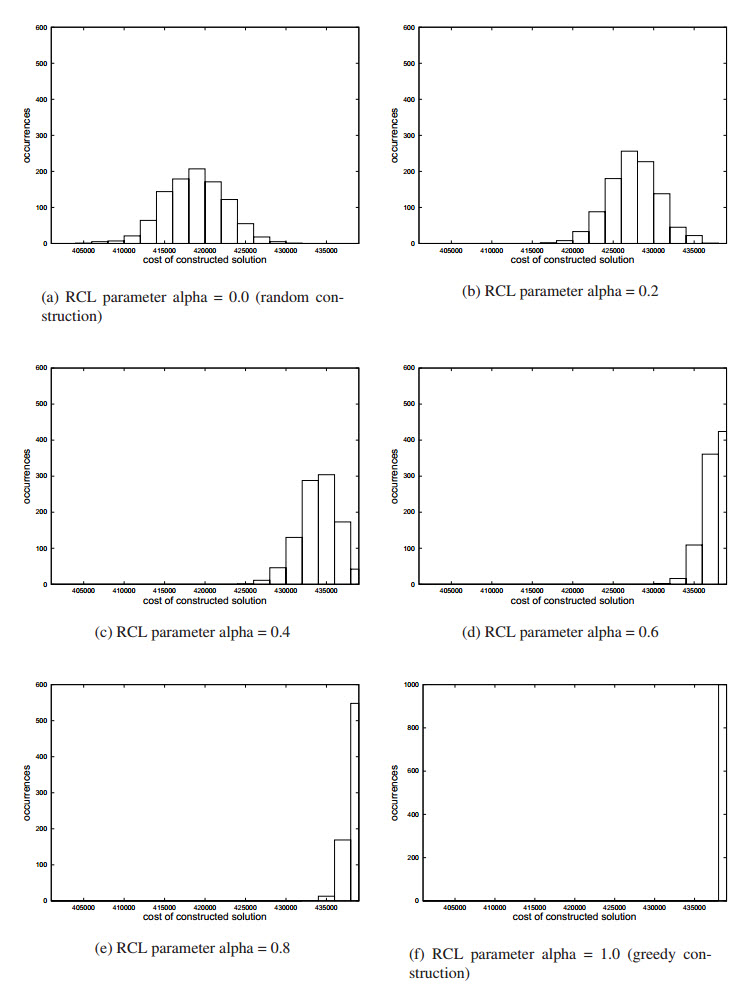
\includegraphics[scale=.75]{images/hinh1_6}
		\end{center}
		\caption{Phân phối giá trị giải pháp của quá trình cấu trúc như một hàm của tham số danh sách RCL $\alpha$ (1000 lần lặp cho mỗi giá trị $\alpha$)}
		\label{refhinh1}
	\end{figure}
\end{center}

\begin{center}
	\begin{figure}[htp]
		\begin{center}
			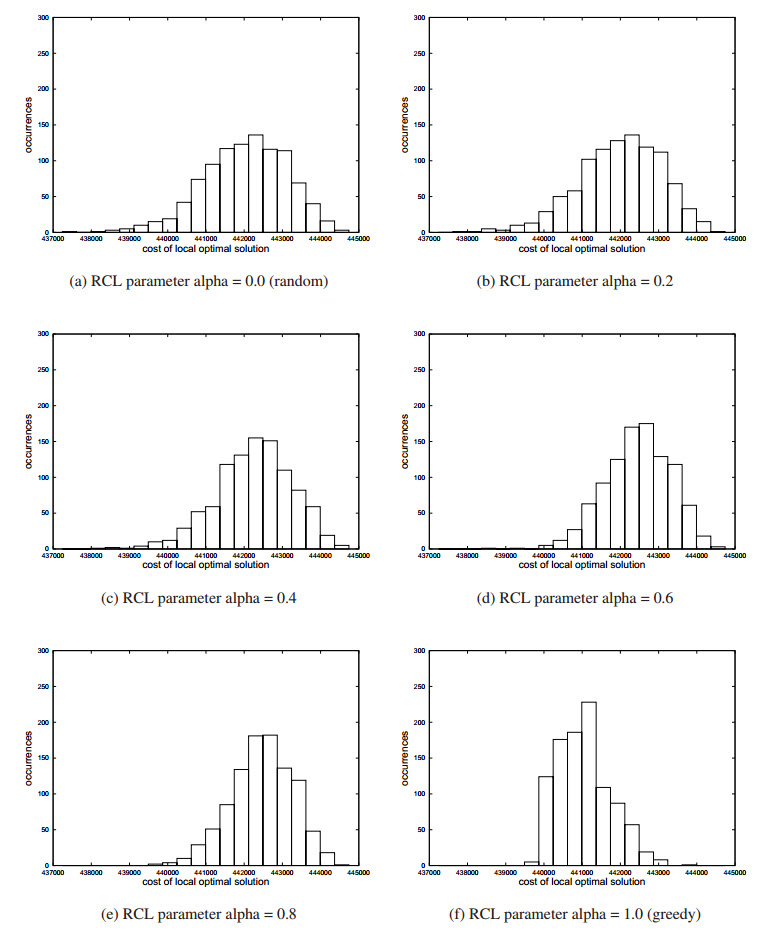
\includegraphics[scale=.75]{images/hinh1_7}
		\end{center}
		\caption{Phân phối giá trị giải pháp của quá trình tìm kiếm địa phương như một hàm của tham số danh sách RCL $\alpha$ (1000 lần lặp cho mỗi giá trị $\alpha$)}
		\label{refhinh2}
	\end{figure}
\end{center}

Với mỗi giá trị của $\alpha$, hình 2.2 thể hiện kết quả thu được khi áp dụng tìm kiếm địa phương tới mỗi 1000 cấu trúc giải pháp. Hình 2.3 tóm tắt các kết quả của thí nghiệm này về sự đa dạng giải pháp, chất lượng và thời gian tính toán. Đầu tiên chúng ta nhận thấy rằng khi phương sai của các giá trị các giải pháp thu được trong gian đoạn đầu tiên càng lớn thì phương sai của tổng thể các giá trị giải pháp càng lớn, xem đồ thị trên. Đồ thị ở giữa minh họa mỗi quan hệ giữa phương sai của giá trị giải pháp và trung bình giá trị giải pháp, và điều này ảnh hưởng như thế nào tới giải pháp tốt nhất tìm được. Không thể chắc chắn rằng GRASP sẽ tìm được giải pháp tối ưu khi giá trị trung bình của giải pháp thấp, thận chí nếu có một phương sai lớn trong tổng thể các giá trị giải pháp, như trường hợp $\alpha$ = 0. Trong trường hợp khác, khi giá trị phương sai nhỏ, GRASP cũng không chắc chắn có thể tìm được giá trị tối ưu, thậm chí khi giá trị trung bình của các giải pháp cao, như trường hợp $\alpha$ = 1. Một giải pháp tốt thường có giá trị trung bình giải pháp cao trong một hiện diện phương sai tương đối lớn, ví dụ: $\alpha$ = 0.8. Đồ thị này cũng chỉ ra rằng khoảnh cách giữa giá trị giải pháp trung bình và giá trị tốt nhất tìm được tăng khi tăng độ tham lam và tính ngẫu nhiên của quá trình xây dựng cấu trúc tham lam ngẫu nhiên thích nghi. Điều này làm cho thời gian chung bình dành cho việc tìm kiếm địa phương tăng lên. giống như đồ thị ở phía dưới. Bình thường, rất nhiều giải pháp GRASP được tạo ra trong cùng một lượng thời gian cần thiết cho thủ tục tối ưu địa phương hội tụ từ một vị trí bắt đầu ngẫu nhiên duy nhất.\\

\begin{center}
	\begin{figure}[htp]
		\begin{center}
			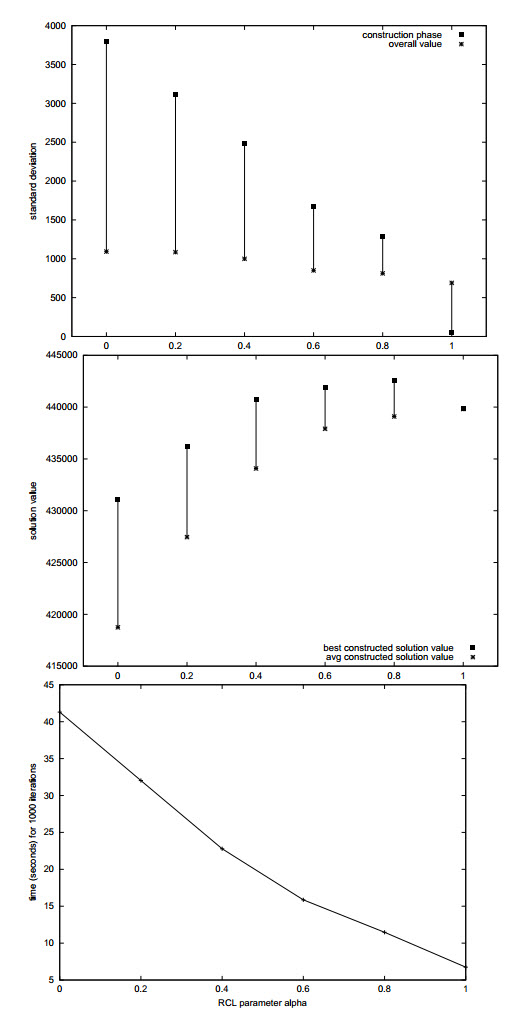
\includegraphics[scale=.75]{images/hinh1_8}
		\end{center}
		\caption{Độ lệch chuẩn của các giải pháp tìm được, giải pháp tốt nhất và giải phải trung bình tìm được, tổng thời gian tìm được như một hàm của tham số RCL $\alpha$ (1000 lần lặp với mỗi giá trị $\alpha$)}
		\label{refhinh3}
	\end{figure}
\end{center}

Các kết quả được minh họa trong hình 2.4 và hình 2.5, về một trường hợp MAXSAT khác với 1000 bước lặp đã chạy. Với mỗi giá trị của $\alpha$ trong khoảng từ 0 tới 1, ta thu được hình 1.9, khoảng cách Hamming trung bình giữa mỗi giải pháp được xây dựng vào cuối giai đoạn đầu tiên và tương ứng với giá trị tối ưu địa phương thu được sau giai đoạn tìm kiếm địa phương. Số trung bình các bước chuyển từ đầu tiên tới cuối cùng. Hình 1.10 tóm tắt giá trị quan sát cho tổng thời gian xử lý và tổng thời gian tìm kiếm. Chú ý rằng, cả hai thời gian đều giảm khi $\alpha$ dần tới 1, tiếp cận tới lựa chọn tham lam. Đặc biệt, thời gian tìm kiếm địa phương khi $\alpha$ = 0 gấp khoảng 2,5 lần trong trương hợp $\alpha$ = 0.9. Lựa chọn giá trị của tham số RCL $\alpha$ rất quan trọng vì nó liên quan tới việc đạt được một sự cân bằng tốt giữa thời gian tính toán và chất lượng của giải pháp.

\begin{center}
	\begin{figure}[htp]
		\begin{center}
			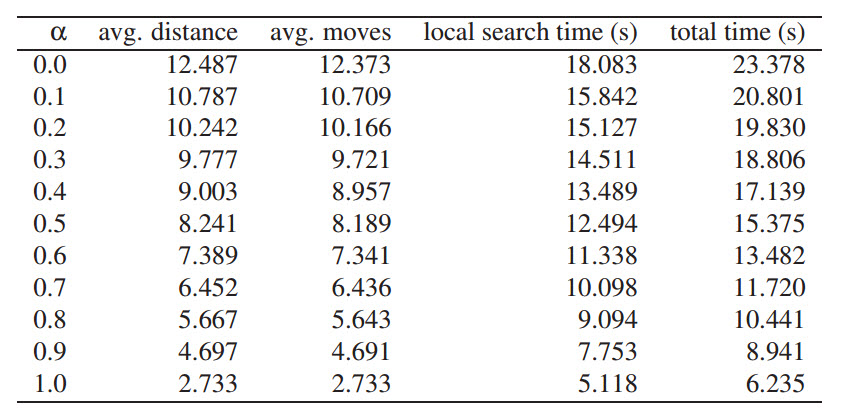
\includegraphics[scale=.65]{images/hinh1_9}
		\end{center}
		\caption{Trung bình số bước di chuyển và thời gian tìm kiếm như một hàm của tham số $\alpha$}
		\label{refhinh4}
	\end{figure}
\end{center}

\begin{center}
	\begin{figure}[htp]
		\begin{center}
			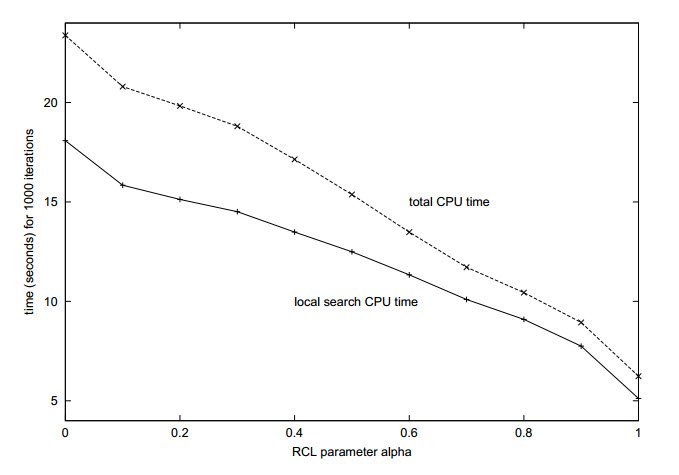
\includegraphics[scale=.55]{images/hinh1_10}
		\end{center}
		\caption{Tổng thời gian CPU và thời gian CPU cho tìm kiếm địa phương như một hàm của tham số RCL $\alpha$ (1000 lần lặp với mỗi giá trị $\alpha$)}
		\label{refhinh5}
	\end{figure}
\end{center}

\chapter{Tổng kết và ứng dụng của giải thuật GRASP}
\section{Tổng kết}
Các kết quả được mô tả ở chương trên phản ánh mô tả thành công của GRASP tới một số lượng lớn các lớp bài toán tối ưu tổ hợp cổ điển cũng như các vấn đề thực tiễn trong các lĩnh vực khác nhau của kinh doanh, khoa học và kỹ thuật.\\
Chương trình GRASP được xây dựng đơn giản bằng việc xây dựng hai khối đơn giản GRASP: thủ tục xây dựng giải pháp và phương pháp tìm kiếm địa phương, thường đã có sẵn. Trái với những gì đã xảy ra với các phương pháp metaheuristics khác như Tabu search, hoặc các giải thuật sinh học, với việc sử dụng một lượng lớn các tham số, phiên bản cơ bản của GRASP chỉ yêu cầu điều chỉnh duy nhất một tham số.\\
Gần đây, giải thuật GRASP cơ bản đã được cải tiến rất nhiều và cho phép cải thiện hơn nữa các giải pháp tìm được như các giải thuật React GRASP, tự động điều chỉnh tham số của danh sách ứng viên hạn chế, biến hàng xóm.
\section{Ứng dụng của giải thuật GRASP}
Ứng dụng đầu tiên của GRASP được mô tả trong các tài liệu về vấn đề tập phủ của Feo và Resende (1989). Một số ứng dụng chính của GRASP trong các lĩnh vực khác nhau:
\begin{itemize}[noitemsep]
	\item Định tuyến: Arguello et al. (1997); Atkinson (1998); Bard et al. (1998); Carreto và Baker (2002); Kontoravdis and Bard (1995);
	\item Logic: Deshpande and Triantaphyllou (1998); Pardalos et al. (1996); Resende và Feo (1996); Resende et al. (1997);
	\item Phủ và phân vùng: Areibi and Vannelli (1997); Arguello et al. (1996); Feo và Resende (1989); Ghosh (1996); Hammer and Rader, Jr. (2001);
	\item Vị trí (location): Abdinnour-Helm and Hadley (2000); Delmaire et al. (1999); Klincewicz (1992); Urban (1998); Urban et al. (2000);
	\item Cực tiểu (minimum): Steiner tree Canuto et al. (1999); Martins et al. (1999; 2000; 1998); Ribeiro et al. (2002);
	\item Tối ưu đồ thị: Abello et al. (1999); Feo et al. (1994); Laguna et al.
	(1994); Pardalos et al. (1999); Resende (1998); Resende and Ribeiro (1997);
	Ribeiro and Resende (1999);
\end{itemize}


%\newpage
%\chapter{Chỉ mục}
%\indexname
\begin{thebibliography}{99}
\bibitem{article1}   Mauricio G. C. Resende, AT\&T Labs – Research, Florham Park, USA “An introduction to GRASP”, 2007
\end{thebibliography}
\newpage
%\chapter{Chỉ mục}
%\indexname

\printindex







\end{document}


